%----------------------------------------------------------------------------
%bb defines the bounding box for the pdf
%viewport defines the area of the pdf used
%in sidewaysfigure the last entry in bb moves the caption toward/away the pic
%in sidewaysfigure the second entry in bb moves the pic toward/away the caption
%----------------------------------------------------------------------------
\begin{figure}
\scalebox{0.8}[0.8]{
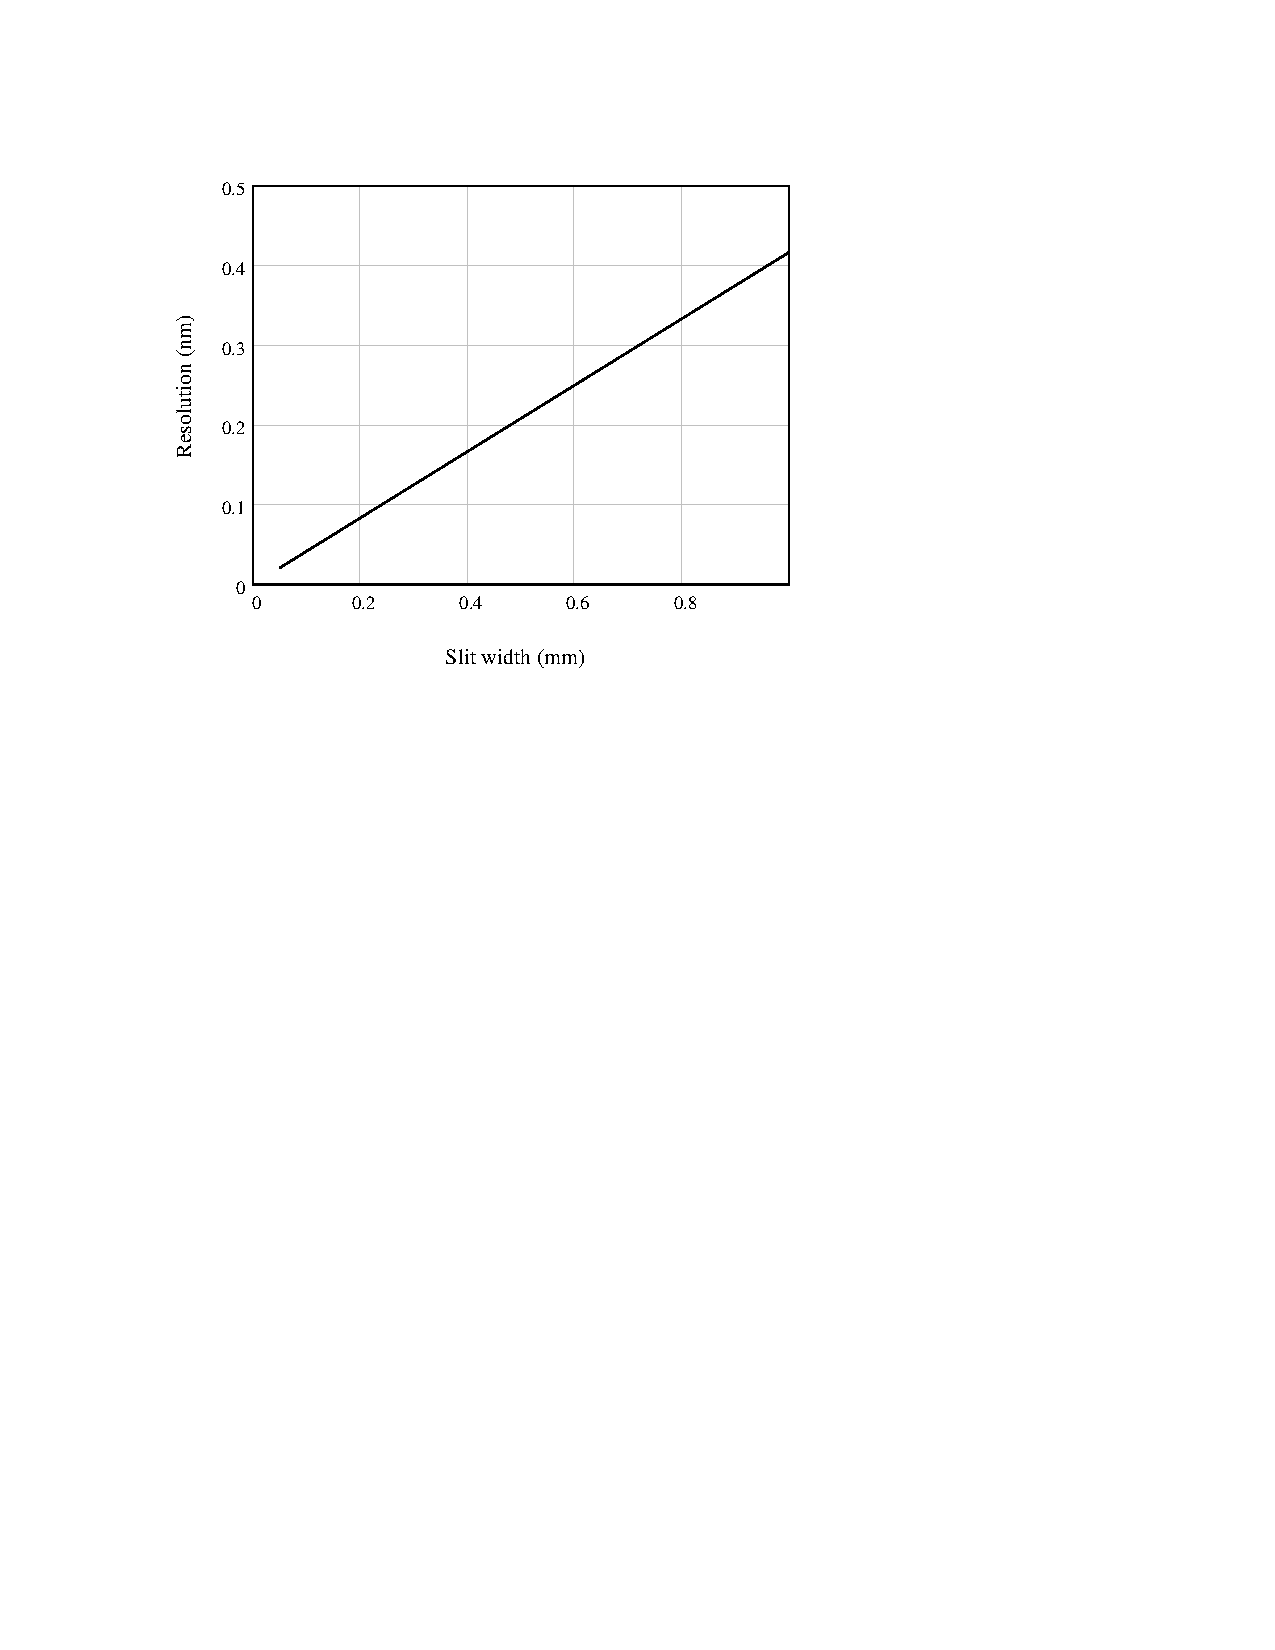
\includegraphics[bb=-30 478 489 700]
{far_nm/far_nm.pdf}
}
\caption[Ideal 1 m monochromator resolution (nm) for large slit widths]{Ideal 1 m monochromator resolution (nm) for large slit widths - Equations \ref{Rayleigh} and \ref{resolvance} imply $\Delta\lambda = a/(2mL\rho)$; here the resolution ($\Delta\lambda$) is ploted for $m=1$, $L=1$ m, and $\rho=1200$ lines per mm.}
\label{far_nm}
\end{figure}
%----------------------------------------------------------------------------
